% To produce pdf under linux, run
% pdflatex hw3.tex

% Credit for this template goes to Dr. Jerry Zhu.

\documentclass{article}
\usepackage[margin=1in]{geometry}
\usepackage{amsmath,amssymb}
\usepackage{bbm}
\usepackage{graphicx}
\usepackage{hyperref}
\usepackage{outlines}
\usepackage{enumitem}
\usepackage{float}
\usepackage{xcolor}
\usepackage{parskip}
\usepackage[skip=0.5\baselineskip]{caption}

\def\bfx{\mathbf x}
\def\R{\mathbb R}
\def\E{\mathbb E}
\def\argmax{\mathrm{argmax}}
\def\argmin{\mathrm{argmin}}


\newenvironment{soln}{
	\leavevmode\color{blue}\ignorespaces
}{}



\title{CS760 Spring 2019 Homework 3}
\author{Due March 28 at 11:59pm}
\date{}
\begin{document}
\maketitle


%%%%%%%%%%%%%%%%%%%%%%%%%%%%%%%%%%%%%%%%%%%%%%%%%%%%%%%%%%%%%%%%%%%%%%%%%
% Insert your name and email here:

Name: Stewart Kerr

Email: shkerr@wisc.edu 

%%%%%%%%%%%%%%%%%%%%%%%%%%%%%%%%%%%%%%%%%%%%%%%%%%%%%%%%%%%%%%%%%%%%%%%%%


\section*{Part 3}

\begin{enumerate}
\item For the logistic regression network built in part 1, plot two curves on one graph, 1) F1 score versus number of epochs on training dataset and 2) F1 score versus number of epochs on testing dataset.

\begin{soln}
See the figure below. I performed logistic regression on both the heart train and test datasets. I used a learning rate of 0.5 and collected data for number of epochs up to 75.

\begin{figure}[h]
\centering
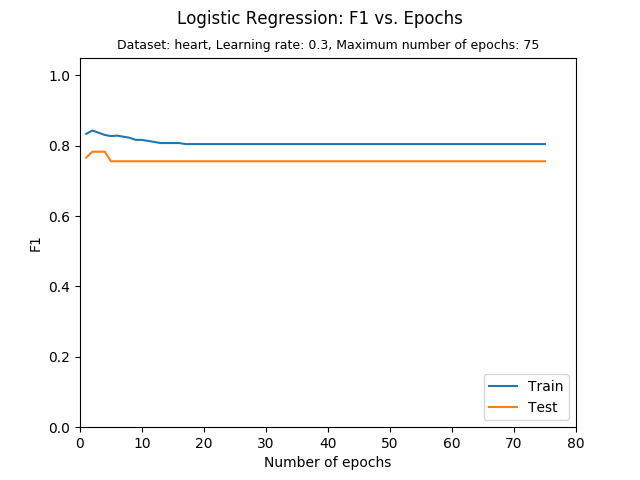
\includegraphics[scale=1]{figs/logistic_f1_curve}
\end{figure}
\end{soln}


\pagebreak
\item Follow the same steps and plot two curves on one graph for the fully connected neural network as described in part 2.

\begin{soln}
See the figure below. Again, I used both the heart train and test datasets to generate F1 scores for a fully-connected neural network with one layer of hidden unites. I used a learning rate of 0.5, a total of 5 hidden units (with one bias unit), and collected data for up to 75 training epochs.

\begin{figure}[h]
\centering
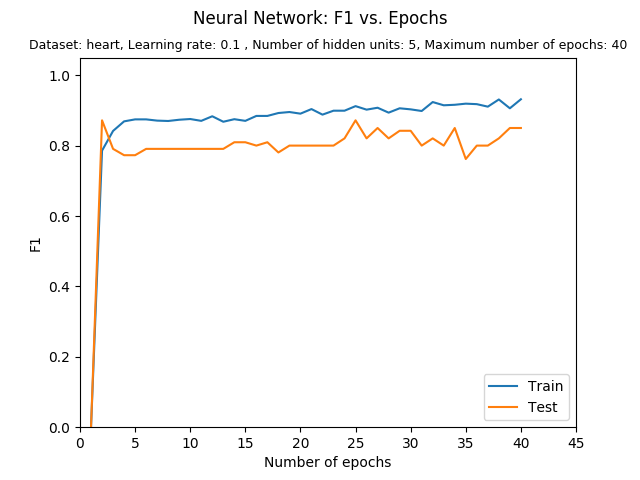
\includegraphics[scale=1]{figs/nnet_f1_curve}
\end{figure}
\end{soln}

\pagebreak
\item Discuss your findings on the above curves. For example, how does the F1 score change when the number of epochs increases, does overfitting occur, does one network outperform the other, etc.

\begin{soln}
\begin{figure}[h]
    \centering
    \begin{minipage}{0.5\textwidth}
        \centering
        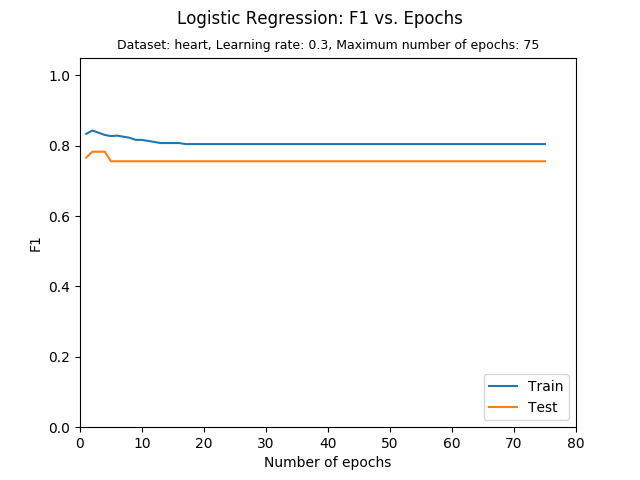
\includegraphics[width=0.9\textwidth]{figs/logistic_f1_curve} 
    \end{minipage}\hfill
    \begin{minipage}{0.5\textwidth}
        \centering
        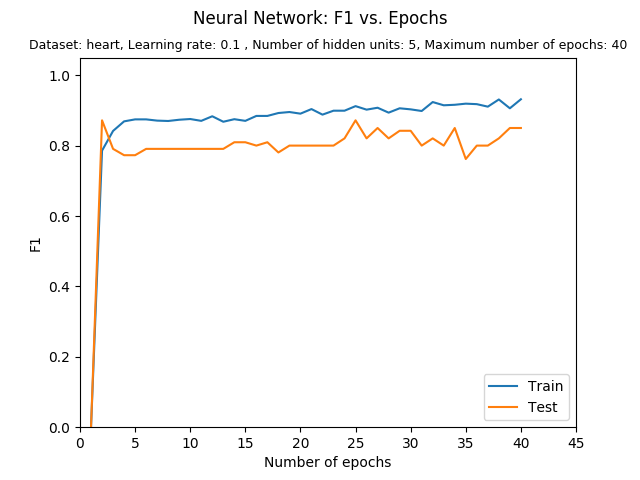
\includegraphics[width=0.9\textwidth]{figs/nnet_f1_curve} 
    \end{minipage}
\end{figure}

I have placed the logistic regression and neural network F1 curves constructed above next to each other. The F1 curve for logistic regression quickly converges for both the test and train datasets with increasing number of epochs (at this particular learning rate). For logistic regression, it appears that performance is actually slightly better with less epochs used in training. The logistic regression classifier performs slightly better on the train dataset than the test dataset, indicating a small amount of overfitting. 

The F1 curve for the neural network also converges relatively quickly but there is a lot more noise for this particular learning rate. Note that decreasing the learning rate would decrease this noise. Unlike the logistic regression curve, the gap between F1 scores for train and F1 scores for test increases as we increase the number of epochs. This indicates that as we increase number of epochs, more overfitting is occuring with the neural network. Thus, we should try to limit the number of epochs used to train (if we use this particular learning rate). 

Now, to compare the two classification methods, it appears that the neural network may sometimes perform slightly better than logistic regression on average, but it also sometimes performs worse. Both methods appear to perform well with only a few number of training epochs. The neural network appears to overfit the data more than logistic regression. I also compared these curves at different learning rates and noticed that lower learning rates (around 0.05) performed better and learning rate appears to have more of an influence on the neural network than logistic regression. If I had to pick a method for this particular problem with our particular restraints, I would probably choose logistic regression because it appears to be a more stable method while still yielding good accuracy.

\end{soln}

\end{enumerate}

\end{document}
]